\documentclass{oci}
\usepackage[utf8]{inputenc}
\usepackage{lipsum}
\usepackage{tikz}

\title{Dados al ataque}
\codename{ataque}

\begin{document}
\begin{problemDescription}
  Ataque es un popular juego de mesa comercializado en Chile por la empresa Hobby.
  El objetivo del juego es conquistar territorios para completar una misión dada
  a cada jugador.
  En cada turno los jugadores deben atacar los territorios enemigos quienes
  intentarán defenderse.

  Para poder atacar al enemigo, un jugador debe lanzar una cierta cantidad de
  dados de acuerdo al número de \emph{ejércitos} que este posea.
  El jugador defensor deberá lanzar la misma cantidad.
  Para saber el resultado del ataque tanto los dados del jugador atacante como
  los del defensor se ordenan de mayor a menor.
  Luego, el mayor dado del atacante es comparado con el mayor dado del defensor.
  El jugador con el peor puntaje entre ambos dados perderá un ejército.
  En caso de haber empate el jugador defensor es quien sale victorioso y el
  atacante pierde un ejército.
  Posteriormente, se procede a comparar el segundo mejor dado del atacante con
  el segundo mejor del defensor y nuevamente perderá un ejército quien haya
  obtenido peor puntaje (resolviendo los empates en favor del defensor).
  Se continúa de esta forma hasta haber comparado todos los pares de dados.
  
  La figura de más abajo muestra un ejemplo donde cada jugador ha lanzado tres
  dados.
  En el ejemplo, el jugador atacante obtuvo un 6 en su dado con mayor puntaje,
  mientras que el defensor un 3, por lo tanto el atacante sale victorioso y el
  defensor pierde un ejército.
  En el siguiente par de dados ambos jugadores obtuvieron el mismo puntaje y por
  lo tanto el defensor sale victorioso y el atacante pierde un ejército.
  Finalmente, en el último par de dados el defensor obtiene mejor puntaje y por
  lo tanto el atacante pierde un ejército.
  En total el jugador atacante pierde 2 ejércitos, mientras que el defensor solo
  pierde 1.
  \begin{center}
  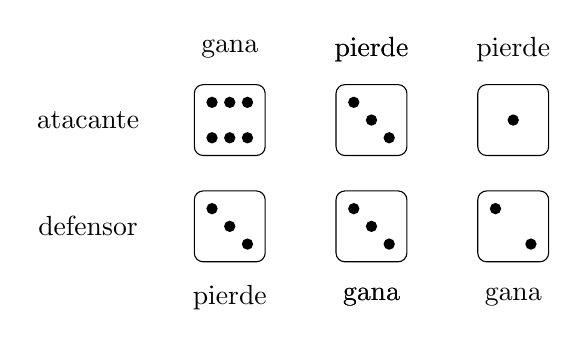
\begin{tikzpicture}[scale=.9]
  \def\one{+(0.00,0.00) circle [radius=0.08]}
  \def\two{+(-.25, .25) circle [radius=0.08]
    +( .25,-.25) circle [radius=0.08]}
  \def\thr{+(-.25, .25) circle [radius=0.08]
    +(0.00,0.00) circle [radius=0.08]
    +( .25,-.25) circle [radius=0.08]}
  \def\fou{+(-.25,-.25) circle [radius=0.08]
    +(-.25, .25) circle [radius=0.08]
    +( .25,-.25) circle [radius=0.08]
    +( .25, .25) circle [radius=0.08]}
  \def\fiv{+(-.25,-.25) circle [radius=0.08]
    +(-.25, .25) circle [radius=0.08]
    +(0.00,0.00) circle [radius=0.08]
    +( .25,-.25) circle [radius=0.08]
    +( .25, .25) circle [radius=0.08]}
  \def\six{+(-.25,-.25) circle [radius=0.08]
    +(-.25, .25) circle [radius=0.08]
    +(0.00,-.25) circle [radius=0.08]
    +(0.00, .25) circle [radius=0.08]
    +( .25,-.25) circle [radius=0.08]
    +( .25, .25) circle [radius=0.08]}
  \def\dice{
    [black,rounded corners=3.2pt]+(-.5,-.5) rectangle +(.5,.5)
  }
  \node at (-2, 0) {atacante};
  % \draw (0, 0) \dice; \fill[rotate around={90:(0,0)}] (0, 0) \six;
  \draw (0, 0) \dice; \fill (0, 0) \six;
  \draw (2, 0) \dice; \fill (2, 0) \thr;
  \draw (4, 0) \dice; \fill (4, 0) \one;


  \node at (-2, -1.5) {defensor};
  \draw (0, -1.5) \dice; \fill (0, -1.5) \thr;
  \draw (2, -1.5) \dice; \fill (2, -1.5) \thr;
  \draw (4, -1.5) \dice; \fill (4, -1.5) \two;
  
  \node at (0, 1) {gana};
  \node at (0, -2.5) {pierde};

  \node at (2, 1) {pierde};
  \node at (2, -2.5) {gana};

  \node at (2, 1) {pierde};
  \node at (2, -2.5) {gana};

  \node at (4, 1) {pierde};
  \node at (4, -2.5) {gana};
  \end{tikzpicture}
  \end{center}

  Debido a su gran popularidad, Hobby está desarrollando una versión electrónica
  del Ataque.
  Lamentablemente están teniendo problemas para implementar el módulo encargado
  de la comparación de los dados.
  Después de todo es una empresa de juegos de mesa y no de programación.
  ?`Podrías ayudarlos?

\end{problemDescription}

\begin{inputDescription}
  La entrada consiste en varias líneas.
  La primera contiene un entero $N$ correspondiente a la cantidad de
  dados lanzados por cada jugador.
  La segunda línea describe los dados lanzados por el jugador
  atacante y contiene $N$ enteros entre 1 y 6 ordenados de mayor a menor.
  Finalmente, la última línea describe los dados lanzados por el jugador defensor de
  la misma forma.
\end{inputDescription}

\begin{outputDescription}
  La salida debe consistir en una única línea con dos enteros $A$ y $D$.
  El entero $A$ debe indicar la cantidad total de ejércitos que perdió el
  jugador atacante y $D$ la cantidad de ejércitos que perdió el jugador
  defensor.
\end{outputDescription}

\begin{scoreDescription}
  \score{40} Se probarán varios casos donde $N=1$.
  \score{60} Se probarán varios casos donde $2\leq N \leq 5$.
\end{scoreDescription}

\begin{sampleDescription}
\sampleIO{sample-1}
\sampleIO{sample-2}
\end{sampleDescription}

\end{document}
